\documentclass[twoside]{book}

% Packages required by doxygen
\usepackage{fixltx2e}
\usepackage{calc}
\usepackage{doxygen}
\usepackage[export]{adjustbox} % also loads graphicx
\usepackage{graphicx}
\usepackage[utf8]{inputenc}
\usepackage{makeidx}
\usepackage{multicol}
\usepackage{multirow}
\PassOptionsToPackage{warn}{textcomp}
\usepackage{textcomp}
\usepackage[nointegrals]{wasysym}
\usepackage[table]{xcolor}

% Font selection
\usepackage[T1]{fontenc}
\usepackage[scaled=.90]{helvet}
\usepackage{courier}
\usepackage{amssymb}
\usepackage{sectsty}
\renewcommand{\familydefault}{\sfdefault}
\allsectionsfont{%
  \fontseries{bc}\selectfont%
  \color{darkgray}%
}
\renewcommand{\DoxyLabelFont}{%
  \fontseries{bc}\selectfont%
  \color{darkgray}%
}
\newcommand{\+}{\discretionary{\mbox{\scriptsize$\hookleftarrow$}}{}{}}

% Page & text layout
\usepackage{geometry}
\geometry{%
  a4paper,%
  top=2.5cm,%
  bottom=2.5cm,%
  left=2.5cm,%
  right=2.5cm%
}
\tolerance=750
\hfuzz=15pt
\hbadness=750
\setlength{\emergencystretch}{15pt}
\setlength{\parindent}{0cm}
\setlength{\parskip}{3ex plus 2ex minus 2ex}
\makeatletter
\renewcommand{\paragraph}{%
  \@startsection{paragraph}{4}{0ex}{-1.0ex}{1.0ex}{%
    \normalfont\normalsize\bfseries\SS@parafont%
  }%
}
\renewcommand{\subparagraph}{%
  \@startsection{subparagraph}{5}{0ex}{-1.0ex}{1.0ex}{%
    \normalfont\normalsize\bfseries\SS@subparafont%
  }%
}
\makeatother

% Headers & footers
\usepackage{fancyhdr}
\pagestyle{fancyplain}
\fancyhead[LE]{\fancyplain{}{\bfseries\thepage}}
\fancyhead[CE]{\fancyplain{}{}}
\fancyhead[RE]{\fancyplain{}{\bfseries\leftmark}}
\fancyhead[LO]{\fancyplain{}{\bfseries\rightmark}}
\fancyhead[CO]{\fancyplain{}{}}
\fancyhead[RO]{\fancyplain{}{\bfseries\thepage}}
\fancyfoot[LE]{\fancyplain{}{}}
\fancyfoot[CE]{\fancyplain{}{}}
\fancyfoot[RE]{\fancyplain{}{\bfseries\scriptsize Generated by Doxygen }}
\fancyfoot[LO]{\fancyplain{}{\bfseries\scriptsize Generated by Doxygen }}
\fancyfoot[CO]{\fancyplain{}{}}
\fancyfoot[RO]{\fancyplain{}{}}
\renewcommand{\footrulewidth}{0.4pt}
\renewcommand{\chaptermark}[1]{%
  \markboth{#1}{}%
}
\renewcommand{\sectionmark}[1]{%
  \markright{\thesection\ #1}%
}

% Indices & bibliography
\usepackage{natbib}
\usepackage[titles]{tocloft}
\setcounter{tocdepth}{3}
\setcounter{secnumdepth}{5}
\makeindex

% Hyperlinks (required, but should be loaded last)
\usepackage{ifpdf}
\ifpdf
  \usepackage[pdftex,pagebackref=true]{hyperref}
\else
  \usepackage[ps2pdf,pagebackref=true]{hyperref}
\fi
\hypersetup{%
  colorlinks=true,%
  linkcolor=blue,%
  citecolor=blue,%
  unicode%
}

% Custom commands
\newcommand{\clearemptydoublepage}{%
  \newpage{\pagestyle{empty}\cleardoublepage}%
}

\usepackage{caption}
\captionsetup{labelsep=space,justification=centering,font={bf},singlelinecheck=off,skip=4pt,position=top}

%===== C O N T E N T S =====

\begin{document}

% Titlepage & ToC
\hypersetup{pageanchor=false,
             bookmarksnumbered=true,
             pdfencoding=unicode
            }
\pagenumbering{alph}
\begin{titlepage}
\vspace*{7cm}
\begin{center}%
{\Large S\+P\+B\+S\+U\+\_\+optimization \\[1ex]\large 1.\+01 }\\
\vspace*{1cm}
{\large Generated by Doxygen 1.8.13}\\
\end{center}
\end{titlepage}
\clearemptydoublepage
\pagenumbering{roman}
\tableofcontents
\clearemptydoublepage
\pagenumbering{arabic}
\hypersetup{pageanchor=true}

%--- Begin generated contents ---
\chapter{Hierarchical Index}
\section{Class Hierarchy}
This inheritance list is sorted roughly, but not completely, alphabetically\+:\begin{DoxyCompactList}
\item \contentsline{section}{A\+R\+EA}{\pageref{class_a_r_e_a}}{}
\begin{DoxyCompactList}
\item \contentsline{section}{Rectangle}{\pageref{class_rectangle}}{}
\end{DoxyCompactList}
\item \contentsline{section}{F\+U\+NC}{\pageref{class_f_u_n_c}}{}
\begin{DoxyCompactList}
\item \contentsline{section}{Ellips}{\pageref{class_ellips}}{}
\item \contentsline{section}{Levi\+N13}{\pageref{class_levi_n13}}{}
\item \contentsline{section}{Wavy}{\pageref{class_wavy}}{}
\end{DoxyCompactList}
\item \contentsline{section}{O\+P\+T\+I\+M\+I\+S\+A\+T\+I\+ON}{\pageref{class_o_p_t_i_m_i_s_a_t_i_o_n}}{}
\begin{DoxyCompactList}
\item \contentsline{section}{Coordinate\+\_\+wise}{\pageref{class_coordinate__wise}}{}
\item \contentsline{section}{Random\+\_\+search}{\pageref{class_random__search}}{}
\end{DoxyCompactList}
\item \contentsline{section}{S\+T\+OP}{\pageref{class_s_t_o_p}}{}
\begin{DoxyCompactList}
\item \contentsline{section}{Arg\+Norm}{\pageref{class_arg_norm}}{}
\item \contentsline{section}{Iterations}{\pageref{class_iterations}}{}
\end{DoxyCompactList}
\end{DoxyCompactList}

\chapter{Class Index}
\section{Class List}
Here are the classes, structs, unions and interfaces with brief descriptions\+:\begin{DoxyCompactList}
\item\contentsline{section}{\hyperlink{class_a_r_e_a}{A\+R\+EA} }{\pageref{class_a_r_e_a}}{}
\item\contentsline{section}{\hyperlink{class_arg_norm}{Arg\+Norm} }{\pageref{class_arg_norm}}{}
\item\contentsline{section}{\hyperlink{class_coordinate__wise}{Coordinate\+\_\+wise} }{\pageref{class_coordinate__wise}}{}
\item\contentsline{section}{\hyperlink{class_ellips}{Ellips} }{\pageref{class_ellips}}{}
\item\contentsline{section}{\hyperlink{class_f_u_n_c}{F\+U\+NC} }{\pageref{class_f_u_n_c}}{}
\item\contentsline{section}{\hyperlink{class_iterations}{Iterations} }{\pageref{class_iterations}}{}
\item\contentsline{section}{\hyperlink{class_levi_n13}{Levi\+N13} }{\pageref{class_levi_n13}}{}
\item\contentsline{section}{\hyperlink{class_o_p_t_i_m_i_s_a_t_i_o_n}{O\+P\+T\+I\+M\+I\+S\+A\+T\+I\+ON} }{\pageref{class_o_p_t_i_m_i_s_a_t_i_o_n}}{}
\item\contentsline{section}{\hyperlink{class_random__search}{Random\+\_\+search} }{\pageref{class_random__search}}{}
\item\contentsline{section}{\hyperlink{class_rectangle}{Rectangle} }{\pageref{class_rectangle}}{}
\item\contentsline{section}{\hyperlink{class_s_t_o_p}{S\+T\+OP} }{\pageref{class_s_t_o_p}}{}
\item\contentsline{section}{\hyperlink{class_wavy}{Wavy} }{\pageref{class_wavy}}{}
\end{DoxyCompactList}

\chapter{Class Documentation}
\hypertarget{class_a_r_e_a}{}\section{A\+R\+EA Class Reference}
\label{class_a_r_e_a}\index{A\+R\+EA@{A\+R\+EA}}


{\ttfamily \#include $<$A\+R\+E\+A.\+h$>$}

Inheritance diagram for A\+R\+EA\+:\begin{figure}[H]
\begin{center}
\leavevmode
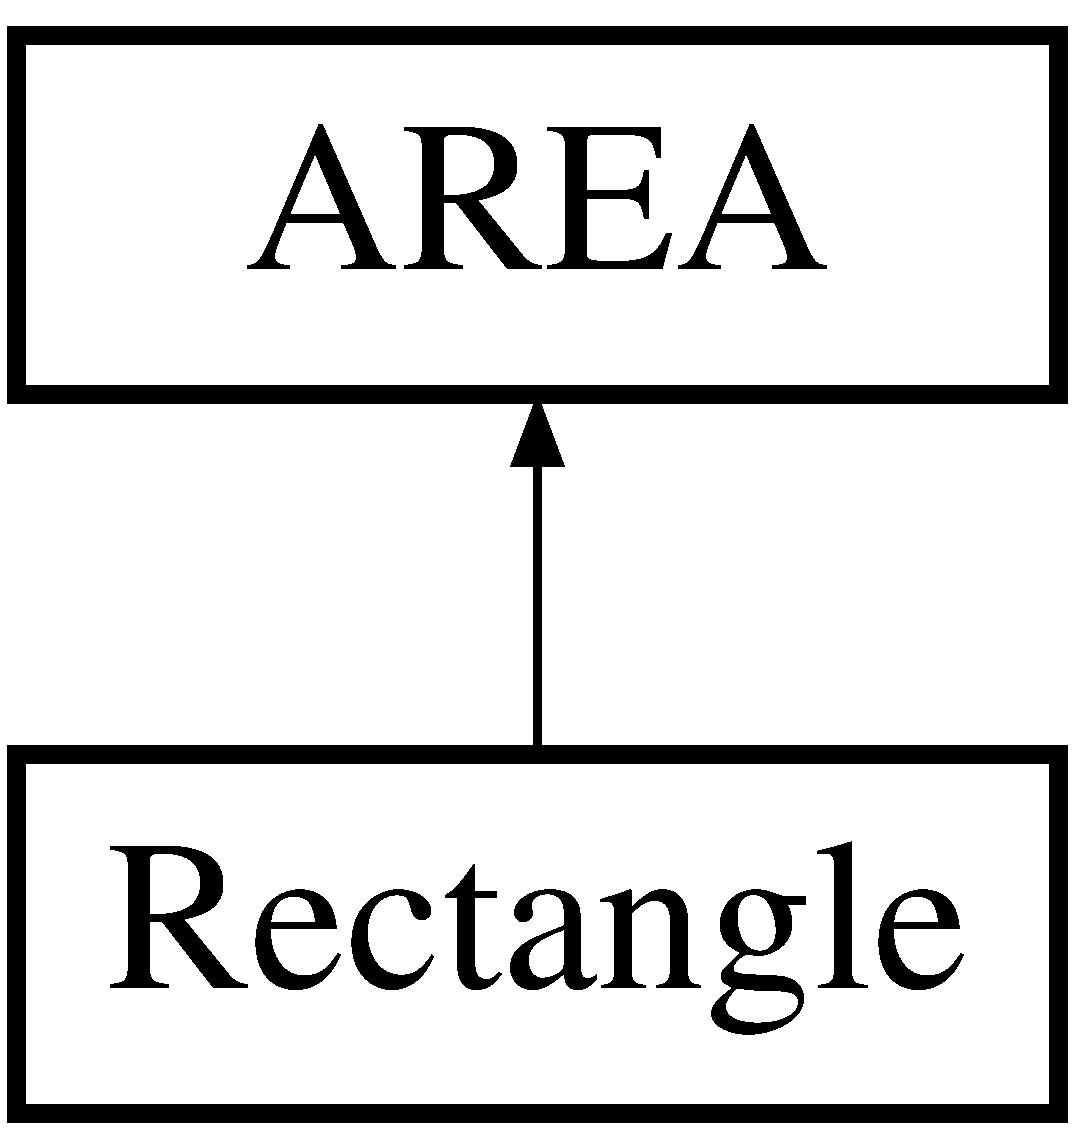
\includegraphics[height=2.000000cm]{class_a_r_e_a}
\end{center}
\end{figure}
\subsection*{Public Member Functions}
\begin{DoxyCompactItemize}
\item 
\mbox{\Hypertarget{class_a_r_e_a_a5319102dccffc30508afbbbfbf572f65}\label{class_a_r_e_a_a5319102dccffc30508afbbbfbf572f65}} 
virtual const std\+::vector$<$ double $>$ {\bfseries get\+\_\+bounds} ()=0
\item 
\mbox{\Hypertarget{class_a_r_e_a_a69de83115e3a6bdbd2bb67bd1608d83a}\label{class_a_r_e_a_a69de83115e3a6bdbd2bb67bd1608d83a}} 
virtual const unsigned int \hyperlink{class_a_r_e_a_a69de83115e3a6bdbd2bb67bd1608d83a}{get\+\_\+dim} (void)=0
\begin{DoxyCompactList}\small\item\em Virtual method to get area bounds. \end{DoxyCompactList}\item 
\mbox{\Hypertarget{class_a_r_e_a_a325ab2d7accb6774bb9f1a34548e0906}\label{class_a_r_e_a_a325ab2d7accb6774bb9f1a34548e0906}} 
virtual const bool \hyperlink{class_a_r_e_a_a325ab2d7accb6774bb9f1a34548e0906}{is\+\_\+in\+\_\+area} (const std\+::vector$<$ double $>$ x)=0
\begin{DoxyCompactList}\small\item\em Virtual method to get dimention. \end{DoxyCompactList}\end{DoxyCompactItemize}
\subsection*{Protected Attributes}
\begin{DoxyCompactItemize}
\item 
std\+::vector$<$ double $>$ \hyperlink{class_a_r_e_a_a9c56910797786fb4d97e42c7829798b7}{\+\_\+bounds}
\end{DoxyCompactItemize}


\subsection{Detailed Description}
Base \hyperlink{class_a_r_e_a}{A\+R\+EA} class 

\subsection{Member Data Documentation}
\mbox{\Hypertarget{class_a_r_e_a_a9c56910797786fb4d97e42c7829798b7}\label{class_a_r_e_a_a9c56910797786fb4d97e42c7829798b7}} 
\index{A\+R\+EA@{A\+R\+EA}!\+\_\+bounds@{\+\_\+bounds}}
\index{\+\_\+bounds@{\+\_\+bounds}!A\+R\+EA@{A\+R\+EA}}
\subsubsection{\texorpdfstring{\+\_\+bounds}{\_bounds}}
{\footnotesize\ttfamily std\+::vector$<$double$>$ A\+R\+E\+A\+::\+\_\+bounds\hspace{0.3cm}{\ttfamily [protected]}}

vector of area bounds 

The documentation for this class was generated from the following file\+:\begin{DoxyCompactItemize}
\item 
spbsu\+\_\+optimization/A\+R\+E\+A.\+h\end{DoxyCompactItemize}

\hypertarget{class_arg_norm}{}\section{Arg\+Norm Class Reference}
\label{class_arg_norm}\index{Arg\+Norm@{Arg\+Norm}}


{\ttfamily \#include $<$S\+T\+O\+P.\+h$>$}

Inheritance diagram for Arg\+Norm\+:\begin{figure}[H]
\begin{center}
\leavevmode
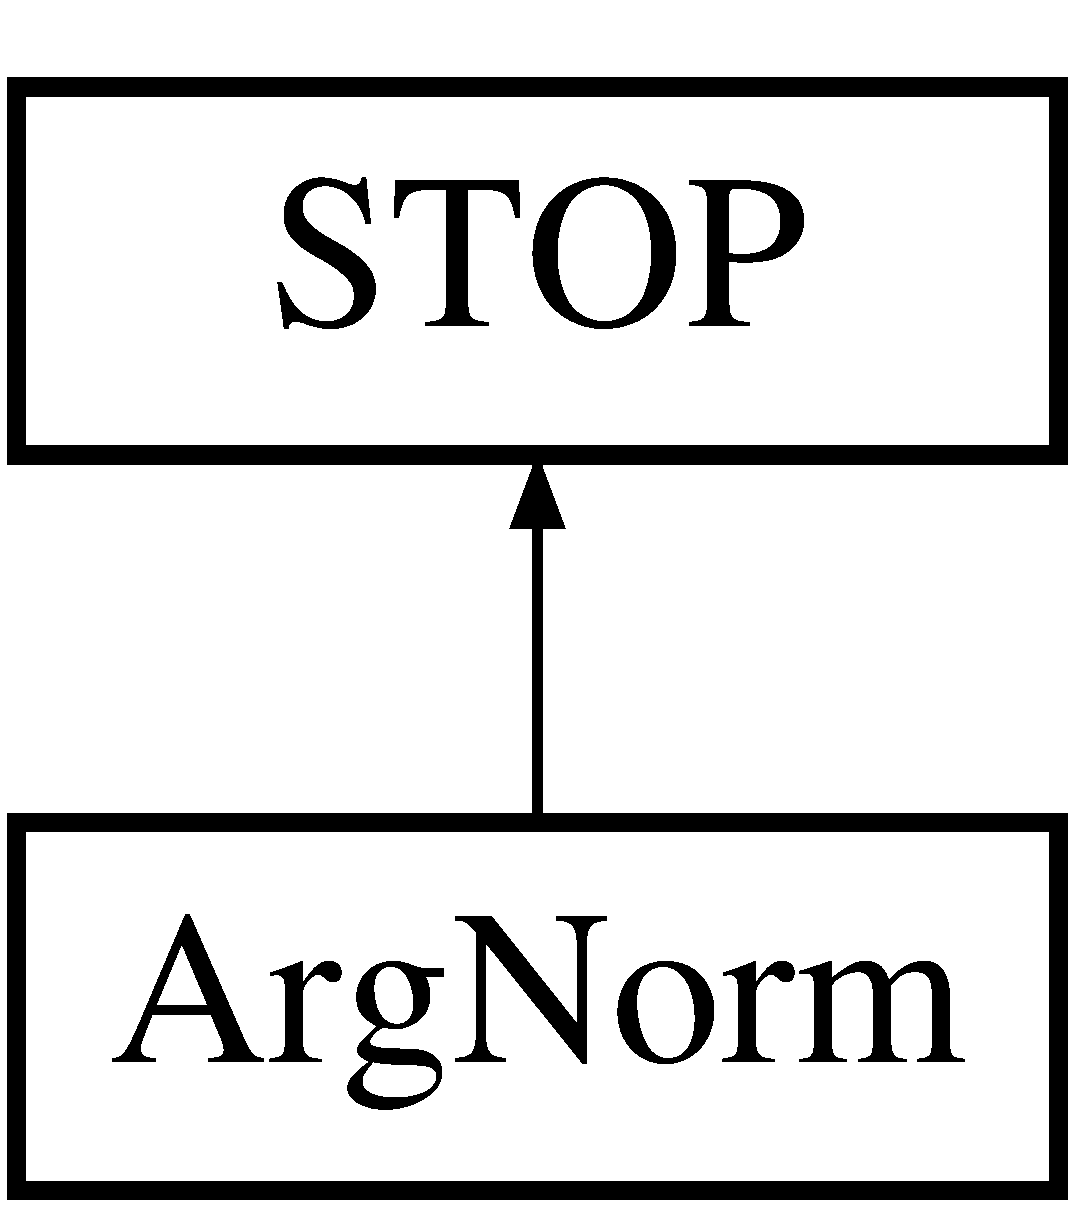
\includegraphics[height=2.000000cm]{class_arg_norm}
\end{center}
\end{figure}
\subsection*{Public Member Functions}
\begin{DoxyCompactItemize}
\item 
\mbox{\Hypertarget{class_arg_norm_ab68ee8dd63445d291bdf9a46cd38aa96}\label{class_arg_norm_ab68ee8dd63445d291bdf9a46cd38aa96}} 
{\bfseries Arg\+Norm} (double eps)
\item 
\mbox{\Hypertarget{class_arg_norm_a360087b606044023e4fc979ddc35cf06}\label{class_arg_norm_a360087b606044023e4fc979ddc35cf06}} 
bool {\bfseries status} ()
\item 
\mbox{\Hypertarget{class_arg_norm_aaaa7006840927462a193a6ed508133e3}\label{class_arg_norm_aaaa7006840927462a193a6ed508133e3}} 
void \hyperlink{class_arg_norm_aaaa7006840927462a193a6ed508133e3}{update} (std\+::vector$<$ double $>$ x\+\_\+curr, std\+::vector$<$ double $>$ x\+\_\+prev, double f\+\_\+curr, double f\+\_\+prev)
\begin{DoxyCompactList}\small\item\em Virtual method to get current status. \end{DoxyCompactList}\end{DoxyCompactItemize}


\subsection{Detailed Description}
Heir of \hyperlink{class_s_t_o_p}{S\+T\+OP} class\+: Stop by vector norm 

The documentation for this class was generated from the following files\+:\begin{DoxyCompactItemize}
\item 
spbsu\+\_\+optimization/S\+T\+O\+P.\+h\item 
spbsu\+\_\+optimization/S\+T\+O\+P.\+cpp\end{DoxyCompactItemize}

\hypertarget{class_coordinate__wise}{}\section{Coordinate\+\_\+wise Class Reference}
\label{class_coordinate__wise}\index{Coordinate\+\_\+wise@{Coordinate\+\_\+wise}}


{\ttfamily \#include $<$O\+P\+T\+I\+M\+I\+S\+A\+T\+I\+O\+N.\+h$>$}

Inheritance diagram for Coordinate\+\_\+wise\+:\begin{figure}[H]
\begin{center}
\leavevmode
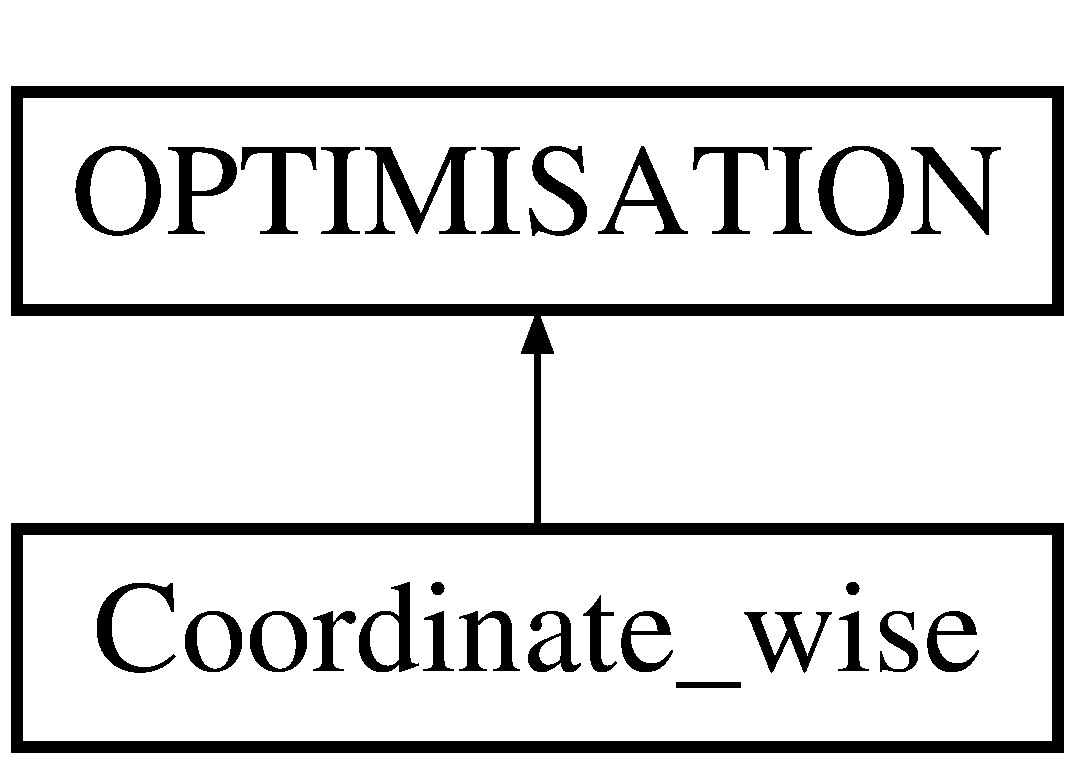
\includegraphics[height=2.000000cm]{class_coordinate__wise}
\end{center}
\end{figure}
\subsection*{Public Member Functions}
\begin{DoxyCompactItemize}
\item 
\mbox{\Hypertarget{class_coordinate__wise_ad14fedb5fb6ad12c8ebb24dd2b91b235}\label{class_coordinate__wise_ad14fedb5fb6ad12c8ebb24dd2b91b235}} 
{\bfseries Coordinate\+\_\+wise} (\hyperlink{class_f_u_n_c}{F\+U\+NC} $\ast$function, \hyperlink{class_a_r_e_a}{A\+R\+EA} $\ast$a, \hyperlink{class_s_t_o_p}{S\+T\+OP} $\ast$stop\+\_\+method, const double N\+\_\+samples=100000, const double p=0.\+8, const double eps=0.\+001)
\item 
\mbox{\Hypertarget{class_coordinate__wise_a7558f5365ca2a1a29385a204389585db}\label{class_coordinate__wise_a7558f5365ca2a1a29385a204389585db}} 
const std\+::vector$<$ double $>$ {\bfseries optimise} (const std\+::vector$<$ double $>$ start)
\item 
\mbox{\Hypertarget{class_coordinate__wise_a01b078176d338e1fd922eb3584900514}\label{class_coordinate__wise_a01b078176d338e1fd922eb3584900514}} 
const std\+::vector$<$ double $>$ \hyperlink{class_coordinate__wise_a01b078176d338e1fd922eb3584900514}{get\+\_\+arg} ()
\begin{DoxyCompactList}\small\item\em Virtual method to argument for min value. \end{DoxyCompactList}\item 
\mbox{\Hypertarget{class_coordinate__wise_a2baa2713d306326b7c322782cdb0dd65}\label{class_coordinate__wise_a2baa2713d306326b7c322782cdb0dd65}} 
const double \hyperlink{class_coordinate__wise_a2baa2713d306326b7c322782cdb0dd65}{get\+\_\+val} ()
\begin{DoxyCompactList}\small\item\em Virtual method to get argument after optimization. \end{DoxyCompactList}\item 
\mbox{\Hypertarget{class_coordinate__wise_ad777100de4f76340bd2b7a03628d0d48}\label{class_coordinate__wise_ad777100de4f76340bd2b7a03628d0d48}} 
const unsigned int \hyperlink{class_coordinate__wise_ad777100de4f76340bd2b7a03628d0d48}{get\+\_\+iterations} ()
\begin{DoxyCompactList}\small\item\em Virtual method to get min value after optimization. \end{DoxyCompactList}\end{DoxyCompactItemize}
\subsection*{Additional Inherited Members}


\subsection{Detailed Description}
Heir of \hyperlink{class_o_p_t_i_m_i_s_a_t_i_o_n}{O\+P\+T\+I\+M\+I\+S\+A\+T\+I\+ON} class\+: Coordinate-\/wise optimization 

The documentation for this class was generated from the following files\+:\begin{DoxyCompactItemize}
\item 
spbsu\+\_\+optimization/O\+P\+T\+I\+M\+I\+S\+A\+T\+I\+O\+N.\+h\item 
spbsu\+\_\+optimization/O\+P\+T\+I\+M\+I\+S\+A\+T\+I\+O\+N.\+cpp\end{DoxyCompactItemize}

\hypertarget{class_ellips}{}\section{Ellips Class Reference}
\label{class_ellips}\index{Ellips@{Ellips}}


{\ttfamily \#include $<$F\+U\+N\+C.\+h$>$}

Inheritance diagram for Ellips\+:\begin{figure}[H]
\begin{center}
\leavevmode
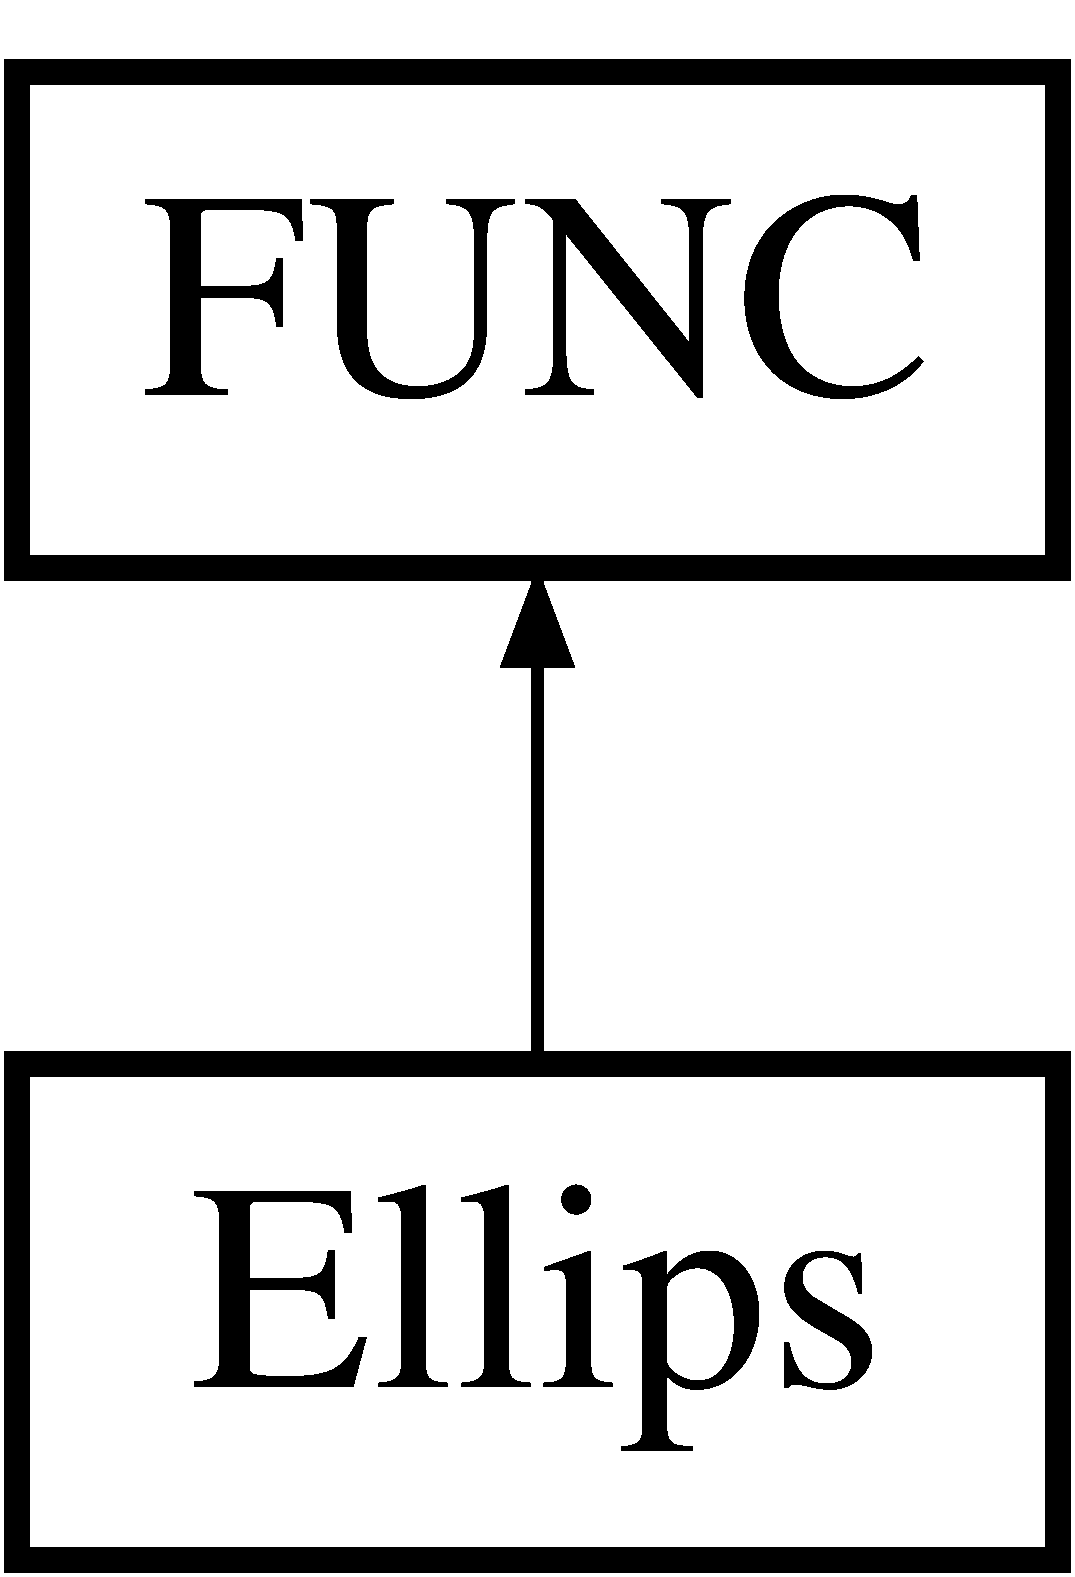
\includegraphics[height=2.000000cm]{class_ellips}
\end{center}
\end{figure}
\subsection*{Public Member Functions}
\begin{DoxyCompactItemize}
\item 
\mbox{\Hypertarget{class_ellips_a037fd4f99158c28dd2c8a92fdfb0cbb7}\label{class_ellips_a037fd4f99158c28dd2c8a92fdfb0cbb7}} 
{\bfseries Ellips} (double a=1, double b=1)
\item 
\mbox{\Hypertarget{class_ellips_ab8df36083101638e1e30896da46893bc}\label{class_ellips_ab8df36083101638e1e30896da46893bc}} 
const double {\bfseries val} (const std\+::vector$<$ double $>$ x)
\item 
\mbox{\Hypertarget{class_ellips_a7297af830c494ecafabac5b1343ee07d}\label{class_ellips_a7297af830c494ecafabac5b1343ee07d}} 
const int \hyperlink{class_ellips_a7297af830c494ecafabac5b1343ee07d}{get\+\_\+dim} (void)
\begin{DoxyCompactList}\small\item\em Virtual method to get value. \end{DoxyCompactList}\end{DoxyCompactItemize}


\subsection{Detailed Description}
Heir of \hyperlink{class_f_u_n_c}{F\+U\+NC} class\+: \hyperlink{class_ellips}{Ellips} function 

The documentation for this class was generated from the following files\+:\begin{DoxyCompactItemize}
\item 
spbsu\+\_\+optimization/F\+U\+N\+C.\+h\item 
spbsu\+\_\+optimization/F\+U\+N\+C.\+cpp\end{DoxyCompactItemize}

\hypertarget{class_f_u_n_c}{}\section{F\+U\+NC Class Reference}
\label{class_f_u_n_c}\index{F\+U\+NC@{F\+U\+NC}}


{\ttfamily \#include $<$F\+U\+N\+C.\+h$>$}

Inheritance diagram for F\+U\+NC\+:\begin{figure}[H]
\begin{center}
\leavevmode
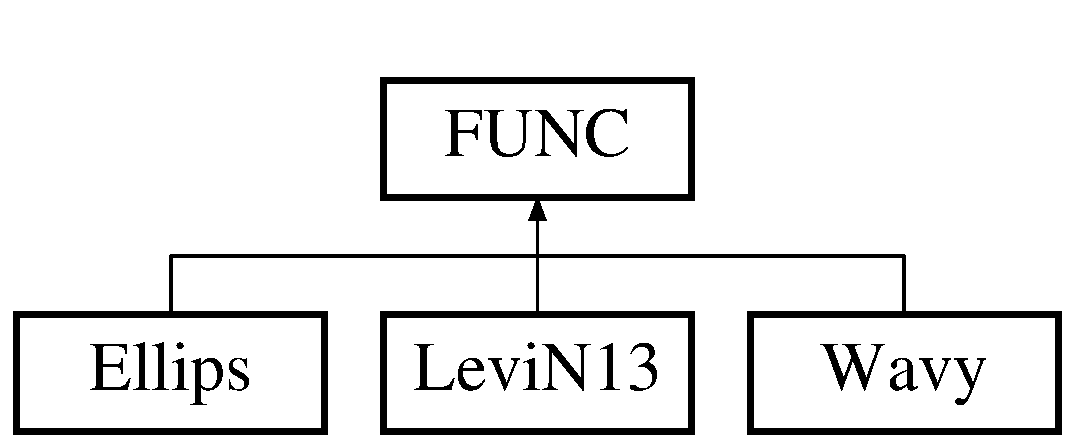
\includegraphics[height=2.000000cm]{class_f_u_n_c}
\end{center}
\end{figure}
\subsection*{Public Member Functions}
\begin{DoxyCompactItemize}
\item 
\mbox{\Hypertarget{class_f_u_n_c_a6355afe1bb2b020af84a1a76ff917a13}\label{class_f_u_n_c_a6355afe1bb2b020af84a1a76ff917a13}} 
virtual const double {\bfseries val} (const std\+::vector$<$ double $>$ x)=0
\item 
\mbox{\Hypertarget{class_f_u_n_c_a0ba70f709ee6569ac2aa0a4ecd147564}\label{class_f_u_n_c_a0ba70f709ee6569ac2aa0a4ecd147564}} 
virtual const int \hyperlink{class_f_u_n_c_a0ba70f709ee6569ac2aa0a4ecd147564}{get\+\_\+dim} (void)=0
\begin{DoxyCompactList}\small\item\em Virtual method to get value. \end{DoxyCompactList}\end{DoxyCompactItemize}


\subsection{Detailed Description}
Base \hyperlink{class_f_u_n_c}{F\+U\+NC} class 

The documentation for this class was generated from the following file\+:\begin{DoxyCompactItemize}
\item 
spbsu\+\_\+optimization/F\+U\+N\+C.\+h\end{DoxyCompactItemize}

\hypertarget{class_iterations}{}\section{Iterations Class Reference}
\label{class_iterations}\index{Iterations@{Iterations}}


{\ttfamily \#include $<$S\+T\+O\+P.\+h$>$}

Inheritance diagram for Iterations\+:\begin{figure}[H]
\begin{center}
\leavevmode
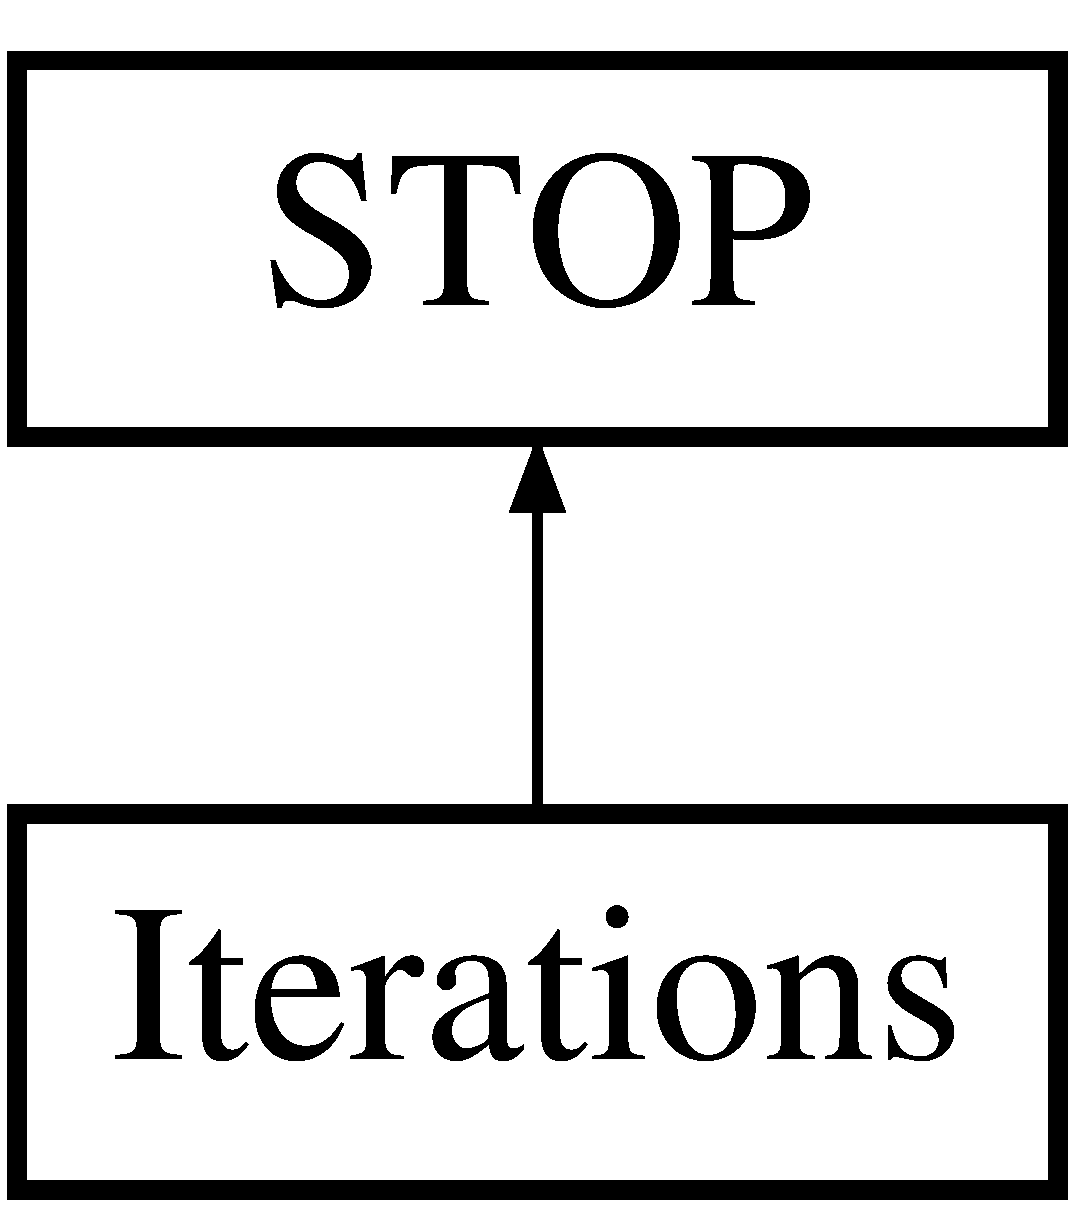
\includegraphics[height=2.000000cm]{class_iterations}
\end{center}
\end{figure}
\subsection*{Public Member Functions}
\begin{DoxyCompactItemize}
\item 
\mbox{\Hypertarget{class_iterations_a3f0d022e3d5a6b45cb7290ff29d01094}\label{class_iterations_a3f0d022e3d5a6b45cb7290ff29d01094}} 
{\bfseries Iterations} (unsigned int M\+AX)
\item 
\mbox{\Hypertarget{class_iterations_a13cee8a7022840c41fd409a489eed513}\label{class_iterations_a13cee8a7022840c41fd409a489eed513}} 
bool {\bfseries status} ()
\item 
\mbox{\Hypertarget{class_iterations_a04b7ede17968ac58df5e36bbd683e37e}\label{class_iterations_a04b7ede17968ac58df5e36bbd683e37e}} 
void \hyperlink{class_iterations_a04b7ede17968ac58df5e36bbd683e37e}{update} (std\+::vector$<$ double $>$ x\+\_\+curr, std\+::vector$<$ double $>$ x\+\_\+prev, double f\+\_\+curr, double f\+\_\+prev)
\begin{DoxyCompactList}\small\item\em Virtual method to get current status. \end{DoxyCompactList}\end{DoxyCompactItemize}


\subsection{Detailed Description}
Heir of \hyperlink{class_s_t_o_p}{S\+T\+OP} class\+: Stop by number of iterarions 

The documentation for this class was generated from the following files\+:\begin{DoxyCompactItemize}
\item 
spbsu\+\_\+optimization/S\+T\+O\+P.\+h\item 
spbsu\+\_\+optimization/S\+T\+O\+P.\+cpp\end{DoxyCompactItemize}

\hypertarget{class_levi_n13}{}\section{Levi\+N13 Class Reference}
\label{class_levi_n13}\index{Levi\+N13@{Levi\+N13}}


{\ttfamily \#include $<$F\+U\+N\+C.\+h$>$}

Inheritance diagram for Levi\+N13\+:\begin{figure}[H]
\begin{center}
\leavevmode
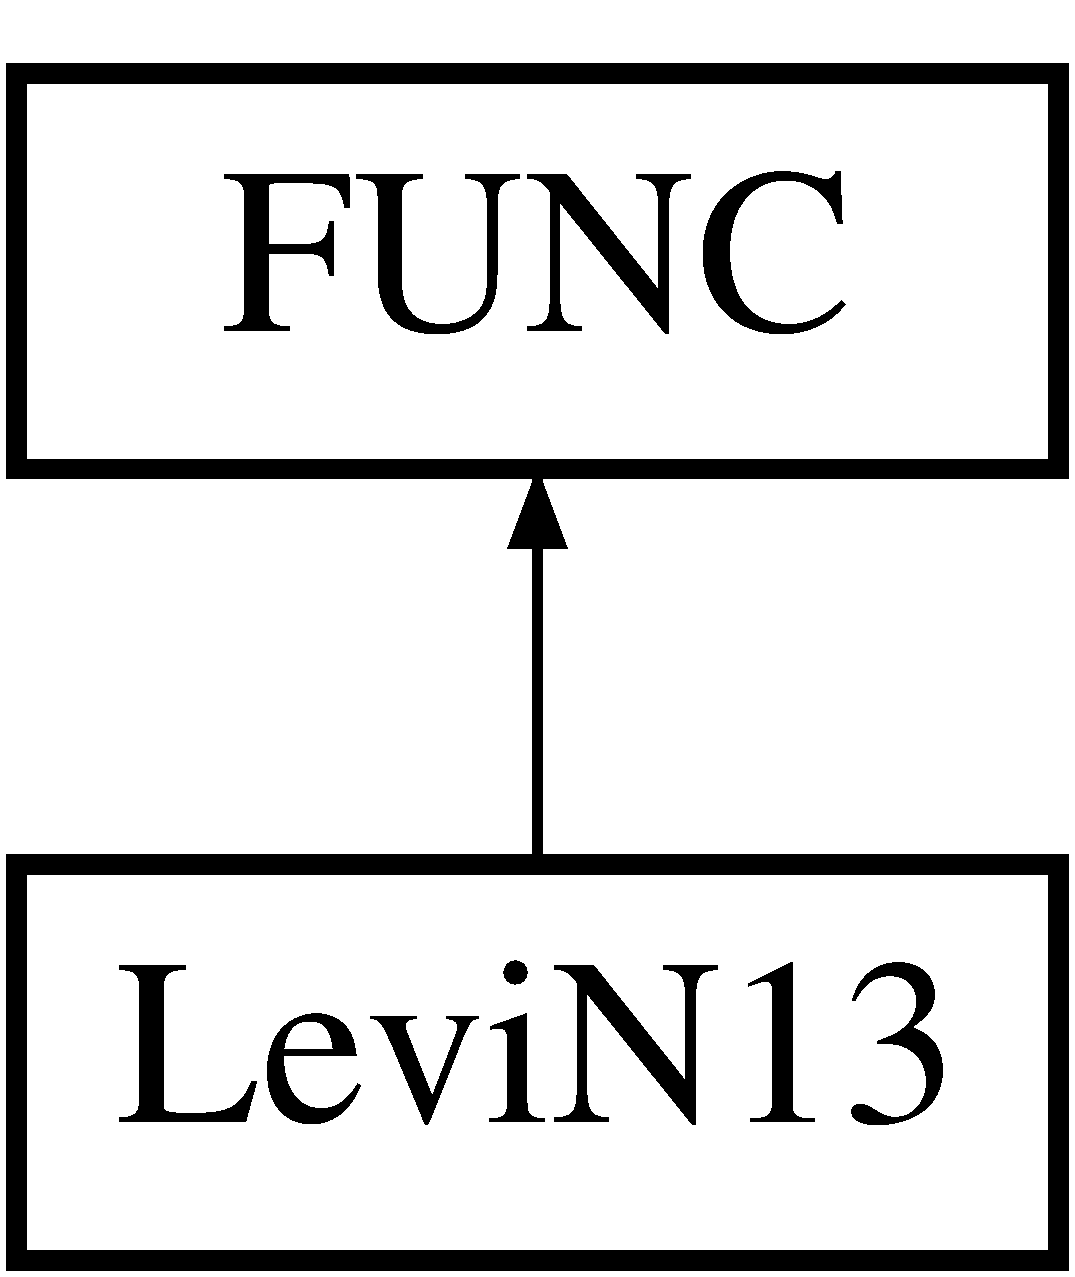
\includegraphics[height=2.000000cm]{class_levi_n13}
\end{center}
\end{figure}
\subsection*{Public Member Functions}
\begin{DoxyCompactItemize}
\item 
\mbox{\Hypertarget{class_levi_n13_ab9abc7db5cfd35367fd60e5abad2fed8}\label{class_levi_n13_ab9abc7db5cfd35367fd60e5abad2fed8}} 
const double {\bfseries val} (const std\+::vector$<$ double $>$ x)
\item 
\mbox{\Hypertarget{class_levi_n13_aaab8c7247ab648e9aed6f535747e8995}\label{class_levi_n13_aaab8c7247ab648e9aed6f535747e8995}} 
const int \hyperlink{class_levi_n13_aaab8c7247ab648e9aed6f535747e8995}{get\+\_\+dim} (void)
\begin{DoxyCompactList}\small\item\em Virtual method to get value. \end{DoxyCompactList}\end{DoxyCompactItemize}


\subsection{Detailed Description}
Heir of \hyperlink{class_f_u_n_c}{F\+U\+NC} class\+: \hyperlink{class_levi_n13}{Levi\+N13} function 

The documentation for this class was generated from the following files\+:\begin{DoxyCompactItemize}
\item 
spbsu\+\_\+optimization/F\+U\+N\+C.\+h\item 
spbsu\+\_\+optimization/F\+U\+N\+C.\+cpp\end{DoxyCompactItemize}

\hypertarget{class_o_p_t_i_m_i_s_a_t_i_o_n}{}\section{O\+P\+T\+I\+M\+I\+S\+A\+T\+I\+ON Class Reference}
\label{class_o_p_t_i_m_i_s_a_t_i_o_n}\index{O\+P\+T\+I\+M\+I\+S\+A\+T\+I\+ON@{O\+P\+T\+I\+M\+I\+S\+A\+T\+I\+ON}}


{\ttfamily \#include $<$O\+P\+T\+I\+M\+I\+S\+A\+T\+I\+O\+N.\+h$>$}

Inheritance diagram for O\+P\+T\+I\+M\+I\+S\+A\+T\+I\+ON\+:\begin{figure}[H]
\begin{center}
\leavevmode
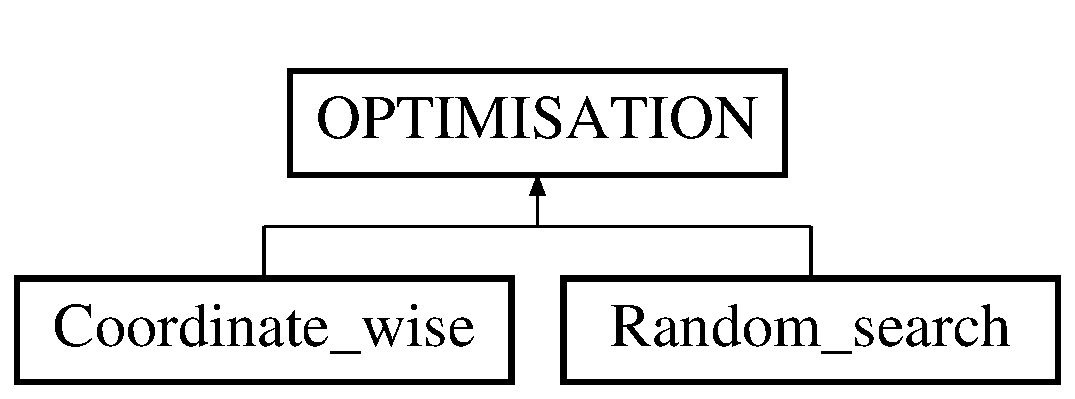
\includegraphics[height=2.000000cm]{class_o_p_t_i_m_i_s_a_t_i_o_n}
\end{center}
\end{figure}
\subsection*{Public Member Functions}
\begin{DoxyCompactItemize}
\item 
\mbox{\Hypertarget{class_o_p_t_i_m_i_s_a_t_i_o_n_a3f2fcfe6f4cf0f58ddbf371f5c8ff7b5}\label{class_o_p_t_i_m_i_s_a_t_i_o_n_a3f2fcfe6f4cf0f58ddbf371f5c8ff7b5}} 
virtual const std\+::vector$<$ double $>$ {\bfseries optimise} (const std\+::vector$<$ double $>$ start)=0
\item 
\mbox{\Hypertarget{class_o_p_t_i_m_i_s_a_t_i_o_n_aacf344bc5597a9e43ac1ab3d7524c99d}\label{class_o_p_t_i_m_i_s_a_t_i_o_n_aacf344bc5597a9e43ac1ab3d7524c99d}} 
virtual const std\+::vector$<$ double $>$ \hyperlink{class_o_p_t_i_m_i_s_a_t_i_o_n_aacf344bc5597a9e43ac1ab3d7524c99d}{get\+\_\+arg} ()=0
\begin{DoxyCompactList}\small\item\em Virtual method to argument for min value. \end{DoxyCompactList}\item 
\mbox{\Hypertarget{class_o_p_t_i_m_i_s_a_t_i_o_n_a82e3d63c255420296cff9d5ac7e0c439}\label{class_o_p_t_i_m_i_s_a_t_i_o_n_a82e3d63c255420296cff9d5ac7e0c439}} 
virtual const double \hyperlink{class_o_p_t_i_m_i_s_a_t_i_o_n_a82e3d63c255420296cff9d5ac7e0c439}{get\+\_\+val} ()=0
\begin{DoxyCompactList}\small\item\em Virtual method to get argument after optimization. \end{DoxyCompactList}\item 
\mbox{\Hypertarget{class_o_p_t_i_m_i_s_a_t_i_o_n_ac45869edc3951dbe68fb0b3293b53c28}\label{class_o_p_t_i_m_i_s_a_t_i_o_n_ac45869edc3951dbe68fb0b3293b53c28}} 
virtual const unsigned int \hyperlink{class_o_p_t_i_m_i_s_a_t_i_o_n_ac45869edc3951dbe68fb0b3293b53c28}{get\+\_\+iterations} ()=0
\begin{DoxyCompactList}\small\item\em Virtual method to get min value after optimization. \end{DoxyCompactList}\end{DoxyCompactItemize}
\subsection*{Protected Attributes}
\begin{DoxyCompactItemize}
\item 
\hyperlink{class_f_u_n_c}{F\+U\+NC} $\ast$ \hyperlink{class_o_p_t_i_m_i_s_a_t_i_o_n_a7301208a647b51b5880ffc1a23da1453}{\+\_\+f}
\item 
\hyperlink{class_a_r_e_a}{A\+R\+EA} $\ast$ \hyperlink{class_o_p_t_i_m_i_s_a_t_i_o_n_ae7b53c1ad284d2da7293acf32dedff33}{\+\_\+area}
\item 
\hyperlink{class_s_t_o_p}{S\+T\+OP} $\ast$ \hyperlink{class_o_p_t_i_m_i_s_a_t_i_o_n_a756cffba62054d4c9f54b8575e0d771e}{\+\_\+stop}
\item 
std\+::vector$<$ double $>$ \hyperlink{class_o_p_t_i_m_i_s_a_t_i_o_n_a049bd3ae26ad1519bbdc81a434e0a886}{\+\_\+curr\+\_\+pos}
\item 
std\+::vector$<$ double $>$ \hyperlink{class_o_p_t_i_m_i_s_a_t_i_o_n_a9fe2a8559d57479f92ade3ea0fe52ef9}{\+\_\+result}
\item 
double \hyperlink{class_o_p_t_i_m_i_s_a_t_i_o_n_ab894cbac492adc44c0731f89e99e8a58}{\+\_\+val}
\item 
unsigned int \hyperlink{class_o_p_t_i_m_i_s_a_t_i_o_n_a7cff0cfa22d26eaf057526b1cc0936a2}{\+\_\+iterations} = 0
\end{DoxyCompactItemize}


\subsection{Detailed Description}
Base \hyperlink{class_o_p_t_i_m_i_s_a_t_i_o_n}{O\+P\+T\+I\+M\+I\+S\+A\+T\+I\+ON} class 

\subsection{Member Data Documentation}
\mbox{\Hypertarget{class_o_p_t_i_m_i_s_a_t_i_o_n_ae7b53c1ad284d2da7293acf32dedff33}\label{class_o_p_t_i_m_i_s_a_t_i_o_n_ae7b53c1ad284d2da7293acf32dedff33}} 
\index{O\+P\+T\+I\+M\+I\+S\+A\+T\+I\+ON@{O\+P\+T\+I\+M\+I\+S\+A\+T\+I\+ON}!\+\_\+area@{\+\_\+area}}
\index{\+\_\+area@{\+\_\+area}!O\+P\+T\+I\+M\+I\+S\+A\+T\+I\+ON@{O\+P\+T\+I\+M\+I\+S\+A\+T\+I\+ON}}
\subsubsection{\texorpdfstring{\+\_\+area}{\_area}}
{\footnotesize\ttfamily \hyperlink{class_a_r_e_a}{A\+R\+EA}$\ast$ O\+P\+T\+I\+M\+I\+S\+A\+T\+I\+O\+N\+::\+\_\+area\hspace{0.3cm}{\ttfamily [protected]}}

pointer to a \hyperlink{class_a_r_e_a}{A\+R\+EA} \mbox{\Hypertarget{class_o_p_t_i_m_i_s_a_t_i_o_n_a049bd3ae26ad1519bbdc81a434e0a886}\label{class_o_p_t_i_m_i_s_a_t_i_o_n_a049bd3ae26ad1519bbdc81a434e0a886}} 
\index{O\+P\+T\+I\+M\+I\+S\+A\+T\+I\+ON@{O\+P\+T\+I\+M\+I\+S\+A\+T\+I\+ON}!\+\_\+curr\+\_\+pos@{\+\_\+curr\+\_\+pos}}
\index{\+\_\+curr\+\_\+pos@{\+\_\+curr\+\_\+pos}!O\+P\+T\+I\+M\+I\+S\+A\+T\+I\+ON@{O\+P\+T\+I\+M\+I\+S\+A\+T\+I\+ON}}
\subsubsection{\texorpdfstring{\+\_\+curr\+\_\+pos}{\_curr\_pos}}
{\footnotesize\ttfamily std\+::vector$<$double$>$ O\+P\+T\+I\+M\+I\+S\+A\+T\+I\+O\+N\+::\+\_\+curr\+\_\+pos\hspace{0.3cm}{\ttfamily [protected]}}

Current position vector \mbox{\Hypertarget{class_o_p_t_i_m_i_s_a_t_i_o_n_a7301208a647b51b5880ffc1a23da1453}\label{class_o_p_t_i_m_i_s_a_t_i_o_n_a7301208a647b51b5880ffc1a23da1453}} 
\index{O\+P\+T\+I\+M\+I\+S\+A\+T\+I\+ON@{O\+P\+T\+I\+M\+I\+S\+A\+T\+I\+ON}!\+\_\+f@{\+\_\+f}}
\index{\+\_\+f@{\+\_\+f}!O\+P\+T\+I\+M\+I\+S\+A\+T\+I\+ON@{O\+P\+T\+I\+M\+I\+S\+A\+T\+I\+ON}}
\subsubsection{\texorpdfstring{\+\_\+f}{\_f}}
{\footnotesize\ttfamily \hyperlink{class_f_u_n_c}{F\+U\+NC}$\ast$ O\+P\+T\+I\+M\+I\+S\+A\+T\+I\+O\+N\+::\+\_\+f\hspace{0.3cm}{\ttfamily [protected]}}

pointer to a \hyperlink{class_f_u_n_c}{F\+U\+NC} \mbox{\Hypertarget{class_o_p_t_i_m_i_s_a_t_i_o_n_a7cff0cfa22d26eaf057526b1cc0936a2}\label{class_o_p_t_i_m_i_s_a_t_i_o_n_a7cff0cfa22d26eaf057526b1cc0936a2}} 
\index{O\+P\+T\+I\+M\+I\+S\+A\+T\+I\+ON@{O\+P\+T\+I\+M\+I\+S\+A\+T\+I\+ON}!\+\_\+iterations@{\+\_\+iterations}}
\index{\+\_\+iterations@{\+\_\+iterations}!O\+P\+T\+I\+M\+I\+S\+A\+T\+I\+ON@{O\+P\+T\+I\+M\+I\+S\+A\+T\+I\+ON}}
\subsubsection{\texorpdfstring{\+\_\+iterations}{\_iterations}}
{\footnotesize\ttfamily unsigned int O\+P\+T\+I\+M\+I\+S\+A\+T\+I\+O\+N\+::\+\_\+iterations = 0\hspace{0.3cm}{\ttfamily [protected]}}

Number of iterations of algorithm \mbox{\Hypertarget{class_o_p_t_i_m_i_s_a_t_i_o_n_a9fe2a8559d57479f92ade3ea0fe52ef9}\label{class_o_p_t_i_m_i_s_a_t_i_o_n_a9fe2a8559d57479f92ade3ea0fe52ef9}} 
\index{O\+P\+T\+I\+M\+I\+S\+A\+T\+I\+ON@{O\+P\+T\+I\+M\+I\+S\+A\+T\+I\+ON}!\+\_\+result@{\+\_\+result}}
\index{\+\_\+result@{\+\_\+result}!O\+P\+T\+I\+M\+I\+S\+A\+T\+I\+ON@{O\+P\+T\+I\+M\+I\+S\+A\+T\+I\+ON}}
\subsubsection{\texorpdfstring{\+\_\+result}{\_result}}
{\footnotesize\ttfamily std\+::vector$<$double$>$ O\+P\+T\+I\+M\+I\+S\+A\+T\+I\+O\+N\+::\+\_\+result\hspace{0.3cm}{\ttfamily [protected]}}

Optimization result vector \mbox{\Hypertarget{class_o_p_t_i_m_i_s_a_t_i_o_n_a756cffba62054d4c9f54b8575e0d771e}\label{class_o_p_t_i_m_i_s_a_t_i_o_n_a756cffba62054d4c9f54b8575e0d771e}} 
\index{O\+P\+T\+I\+M\+I\+S\+A\+T\+I\+ON@{O\+P\+T\+I\+M\+I\+S\+A\+T\+I\+ON}!\+\_\+stop@{\+\_\+stop}}
\index{\+\_\+stop@{\+\_\+stop}!O\+P\+T\+I\+M\+I\+S\+A\+T\+I\+ON@{O\+P\+T\+I\+M\+I\+S\+A\+T\+I\+ON}}
\subsubsection{\texorpdfstring{\+\_\+stop}{\_stop}}
{\footnotesize\ttfamily \hyperlink{class_s_t_o_p}{S\+T\+OP}$\ast$ O\+P\+T\+I\+M\+I\+S\+A\+T\+I\+O\+N\+::\+\_\+stop\hspace{0.3cm}{\ttfamily [protected]}}

pointer to a \hyperlink{class_s_t_o_p}{S\+T\+OP} \mbox{\Hypertarget{class_o_p_t_i_m_i_s_a_t_i_o_n_ab894cbac492adc44c0731f89e99e8a58}\label{class_o_p_t_i_m_i_s_a_t_i_o_n_ab894cbac492adc44c0731f89e99e8a58}} 
\index{O\+P\+T\+I\+M\+I\+S\+A\+T\+I\+ON@{O\+P\+T\+I\+M\+I\+S\+A\+T\+I\+ON}!\+\_\+val@{\+\_\+val}}
\index{\+\_\+val@{\+\_\+val}!O\+P\+T\+I\+M\+I\+S\+A\+T\+I\+ON@{O\+P\+T\+I\+M\+I\+S\+A\+T\+I\+ON}}
\subsubsection{\texorpdfstring{\+\_\+val}{\_val}}
{\footnotesize\ttfamily double O\+P\+T\+I\+M\+I\+S\+A\+T\+I\+O\+N\+::\+\_\+val\hspace{0.3cm}{\ttfamily [protected]}}

\hyperlink{class_f_u_n_c}{F\+U\+NC} value of optimization result vector 

The documentation for this class was generated from the following file\+:\begin{DoxyCompactItemize}
\item 
spbsu\+\_\+optimization/O\+P\+T\+I\+M\+I\+S\+A\+T\+I\+O\+N.\+h\end{DoxyCompactItemize}

\hypertarget{class_random__search}{}\section{Random\+\_\+search Class Reference}
\label{class_random__search}\index{Random\+\_\+search@{Random\+\_\+search}}


{\ttfamily \#include $<$O\+P\+T\+I\+M\+I\+S\+A\+T\+I\+O\+N.\+h$>$}

Inheritance diagram for Random\+\_\+search\+:\begin{figure}[H]
\begin{center}
\leavevmode
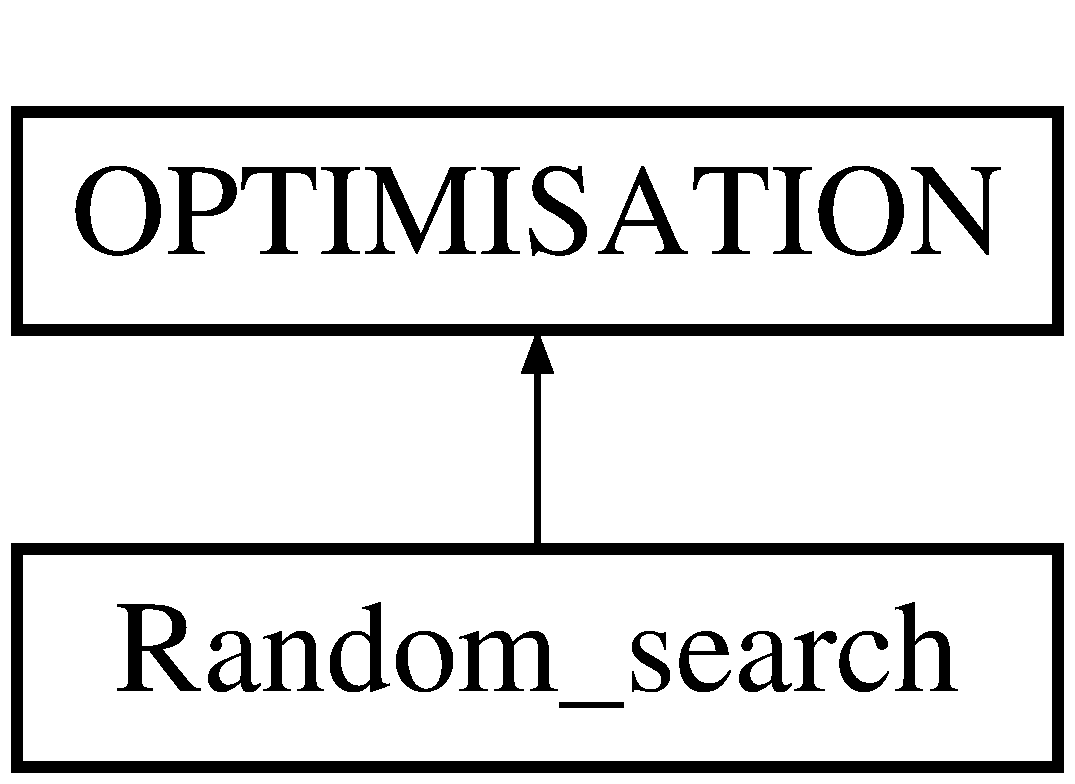
\includegraphics[height=2.000000cm]{class_random__search}
\end{center}
\end{figure}
\subsection*{Public Member Functions}
\begin{DoxyCompactItemize}
\item 
\mbox{\Hypertarget{class_random__search_a727a80d38d90bc60d388615fc36bf422}\label{class_random__search_a727a80d38d90bc60d388615fc36bf422}} 
{\bfseries Random\+\_\+search} (\hyperlink{class_f_u_n_c}{F\+U\+NC} $\ast$function, \hyperlink{class_a_r_e_a}{A\+R\+EA} $\ast$a, \hyperlink{class_s_t_o_p}{S\+T\+OP} $\ast$stop\+\_\+method, const double p=0.\+8, const double eps=0.\+0000001)
\item 
\mbox{\Hypertarget{class_random__search_a82bffda766b580ece0b5ec259e220fa6}\label{class_random__search_a82bffda766b580ece0b5ec259e220fa6}} 
const std\+::vector$<$ double $>$ {\bfseries optimise} (const std\+::vector$<$ double $>$ start)
\item 
\mbox{\Hypertarget{class_random__search_a1fef87ecbb840f70e4703383422ba3ec}\label{class_random__search_a1fef87ecbb840f70e4703383422ba3ec}} 
const std\+::vector$<$ double $>$ \hyperlink{class_random__search_a1fef87ecbb840f70e4703383422ba3ec}{get\+\_\+arg} ()
\begin{DoxyCompactList}\small\item\em Virtual method to argument for min value. \end{DoxyCompactList}\item 
\mbox{\Hypertarget{class_random__search_a7aa1969de56bb81cfc6f0ac5d81080e9}\label{class_random__search_a7aa1969de56bb81cfc6f0ac5d81080e9}} 
const double \hyperlink{class_random__search_a7aa1969de56bb81cfc6f0ac5d81080e9}{get\+\_\+val} ()
\begin{DoxyCompactList}\small\item\em Virtual method to get argument after optimization. \end{DoxyCompactList}\item 
\mbox{\Hypertarget{class_random__search_af05aca1c09c966e863fdac963ebb8641}\label{class_random__search_af05aca1c09c966e863fdac963ebb8641}} 
const unsigned int \hyperlink{class_random__search_af05aca1c09c966e863fdac963ebb8641}{get\+\_\+iterations} ()
\begin{DoxyCompactList}\small\item\em Virtual method to get min value after optimization. \end{DoxyCompactList}\end{DoxyCompactItemize}
\subsection*{Additional Inherited Members}


\subsection{Detailed Description}
Heir of \hyperlink{class_o_p_t_i_m_i_s_a_t_i_o_n}{O\+P\+T\+I\+M\+I\+S\+A\+T\+I\+ON} class\+: \hyperlink{class_random__search}{Random\+\_\+search} optimization 

The documentation for this class was generated from the following files\+:\begin{DoxyCompactItemize}
\item 
spbsu\+\_\+optimization/O\+P\+T\+I\+M\+I\+S\+A\+T\+I\+O\+N.\+h\item 
spbsu\+\_\+optimization/O\+P\+T\+I\+M\+I\+S\+A\+T\+I\+O\+N.\+cpp\end{DoxyCompactItemize}

\hypertarget{class_rectangle}{}\section{Rectangle Class Reference}
\label{class_rectangle}\index{Rectangle@{Rectangle}}


{\ttfamily \#include $<$A\+R\+E\+A.\+h$>$}

Inheritance diagram for Rectangle\+:\begin{figure}[H]
\begin{center}
\leavevmode
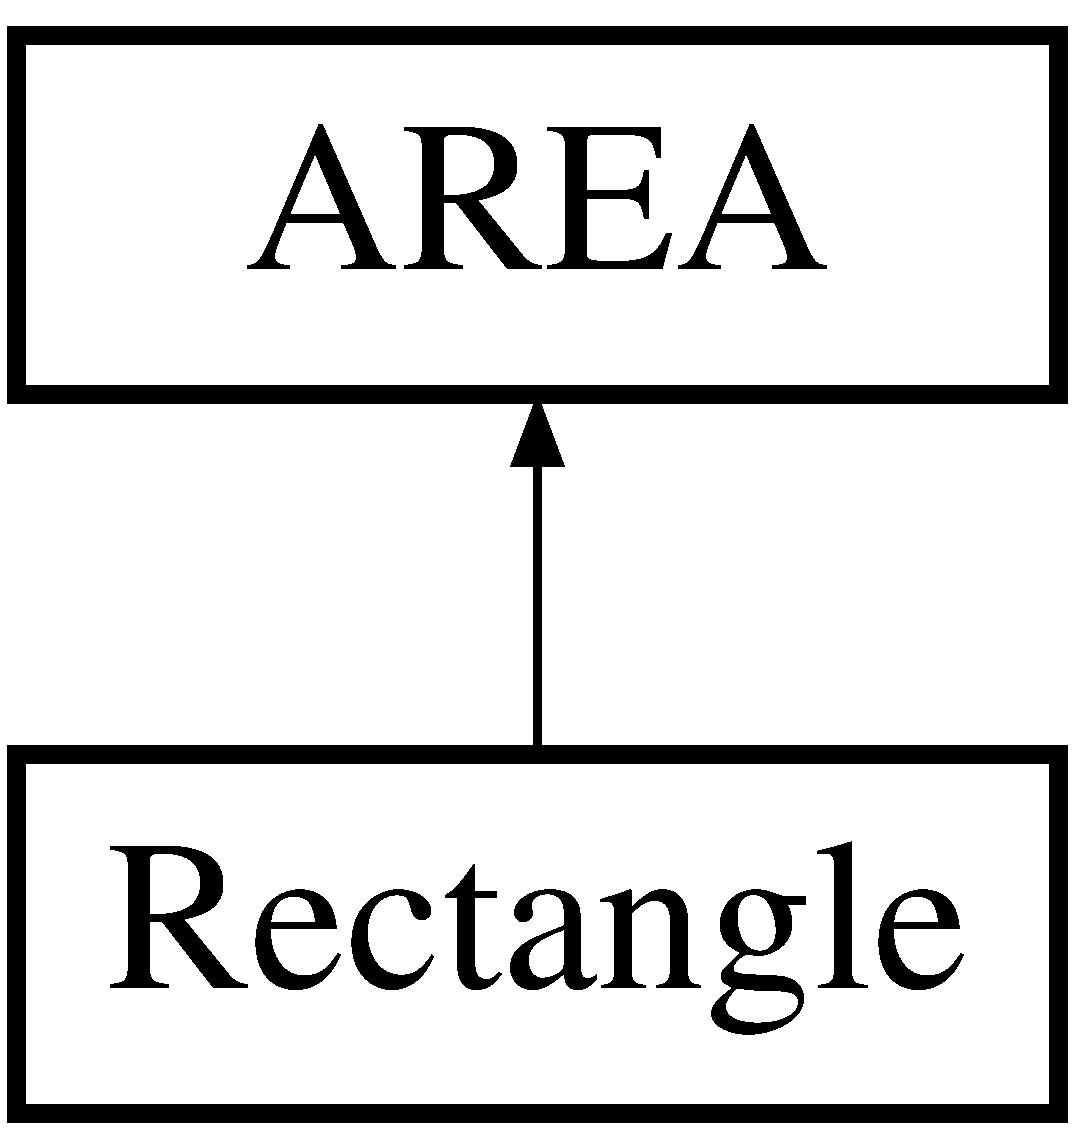
\includegraphics[height=2.000000cm]{class_rectangle}
\end{center}
\end{figure}
\subsection*{Public Member Functions}
\begin{DoxyCompactItemize}
\item 
\mbox{\Hypertarget{class_rectangle_a53b752170e408da7f54037f92f6fbf1b}\label{class_rectangle_a53b752170e408da7f54037f92f6fbf1b}} 
{\bfseries Rectangle} (double a1, double a2, double b1, double b2)
\item 
\mbox{\Hypertarget{class_rectangle_a1441ece4619a41086d4fd9210d8936e8}\label{class_rectangle_a1441ece4619a41086d4fd9210d8936e8}} 
const bool \hyperlink{class_rectangle_a1441ece4619a41086d4fd9210d8936e8}{is\+\_\+in\+\_\+area} (const std\+::vector$<$ double $>$ x)
\begin{DoxyCompactList}\small\item\em \hyperlink{class_rectangle}{Rectangle} area constructor. \end{DoxyCompactList}\item 
\mbox{\Hypertarget{class_rectangle_ab76d97c703e0d99dd625f8f8b43c683a}\label{class_rectangle_ab76d97c703e0d99dd625f8f8b43c683a}} 
const unsigned int \hyperlink{class_rectangle_ab76d97c703e0d99dd625f8f8b43c683a}{get\+\_\+dim} ()
\begin{DoxyCompactList}\small\item\em Virtual method to check if vector is in area of rectangle. \end{DoxyCompactList}\item 
\mbox{\Hypertarget{class_rectangle_a39c267d74f3c82689f2e22b8206afd35}\label{class_rectangle_a39c267d74f3c82689f2e22b8206afd35}} 
const std\+::vector$<$ double $>$ \hyperlink{class_rectangle_a39c267d74f3c82689f2e22b8206afd35}{get\+\_\+bounds} ()
\begin{DoxyCompactList}\small\item\em Virtual method to get dimention of rectangle. \end{DoxyCompactList}\end{DoxyCompactItemize}
\subsection*{Additional Inherited Members}


\subsection{Detailed Description}
Heir of \hyperlink{class_a_r_e_a}{A\+R\+EA} class\+: \hyperlink{class_rectangle}{Rectangle} 

The documentation for this class was generated from the following files\+:\begin{DoxyCompactItemize}
\item 
spbsu\+\_\+optimization/A\+R\+E\+A.\+h\item 
spbsu\+\_\+optimization/A\+R\+E\+A.\+cpp\end{DoxyCompactItemize}

\hypertarget{class_s_t_o_p}{}\section{S\+T\+OP Class Reference}
\label{class_s_t_o_p}\index{S\+T\+OP@{S\+T\+OP}}


{\ttfamily \#include $<$S\+T\+O\+P.\+h$>$}

Inheritance diagram for S\+T\+OP\+:\begin{figure}[H]
\begin{center}
\leavevmode
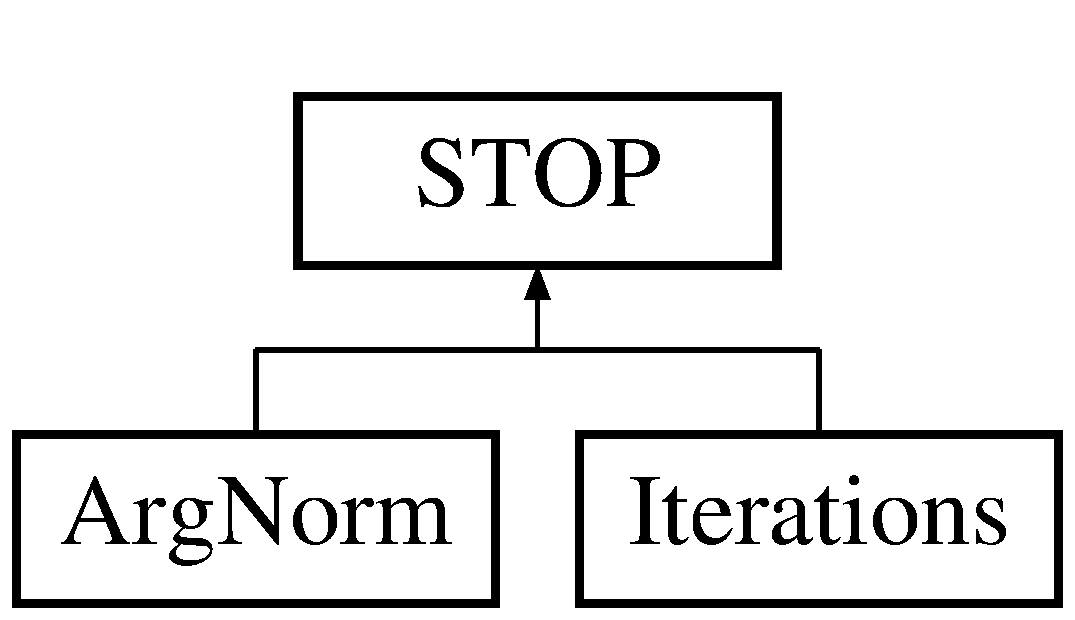
\includegraphics[height=2.000000cm]{class_s_t_o_p}
\end{center}
\end{figure}
\subsection*{Public Member Functions}
\begin{DoxyCompactItemize}
\item 
\mbox{\Hypertarget{class_s_t_o_p_a68218a1646b557bfce7bd9ce5fba94b8}\label{class_s_t_o_p_a68218a1646b557bfce7bd9ce5fba94b8}} 
virtual bool {\bfseries status} ()=0
\item 
\mbox{\Hypertarget{class_s_t_o_p_a0eb3d0b3458f6d5d5071338983ce0782}\label{class_s_t_o_p_a0eb3d0b3458f6d5d5071338983ce0782}} 
virtual void \hyperlink{class_s_t_o_p_a0eb3d0b3458f6d5d5071338983ce0782}{update} (std\+::vector$<$ double $>$ x\+\_\+curr, std\+::vector$<$ double $>$ x\+\_\+prev, double f\+\_\+curr, double f\+\_\+prev)=0
\begin{DoxyCompactList}\small\item\em Virtual method to get current status. \end{DoxyCompactList}\end{DoxyCompactItemize}


\subsection{Detailed Description}
Base \hyperlink{class_s_t_o_p}{S\+T\+OP} class 

The documentation for this class was generated from the following file\+:\begin{DoxyCompactItemize}
\item 
spbsu\+\_\+optimization/S\+T\+O\+P.\+h\end{DoxyCompactItemize}

\hypertarget{class_wavy}{}\section{Wavy Class Reference}
\label{class_wavy}\index{Wavy@{Wavy}}


{\ttfamily \#include $<$F\+U\+N\+C.\+h$>$}

Inheritance diagram for Wavy\+:\begin{figure}[H]
\begin{center}
\leavevmode
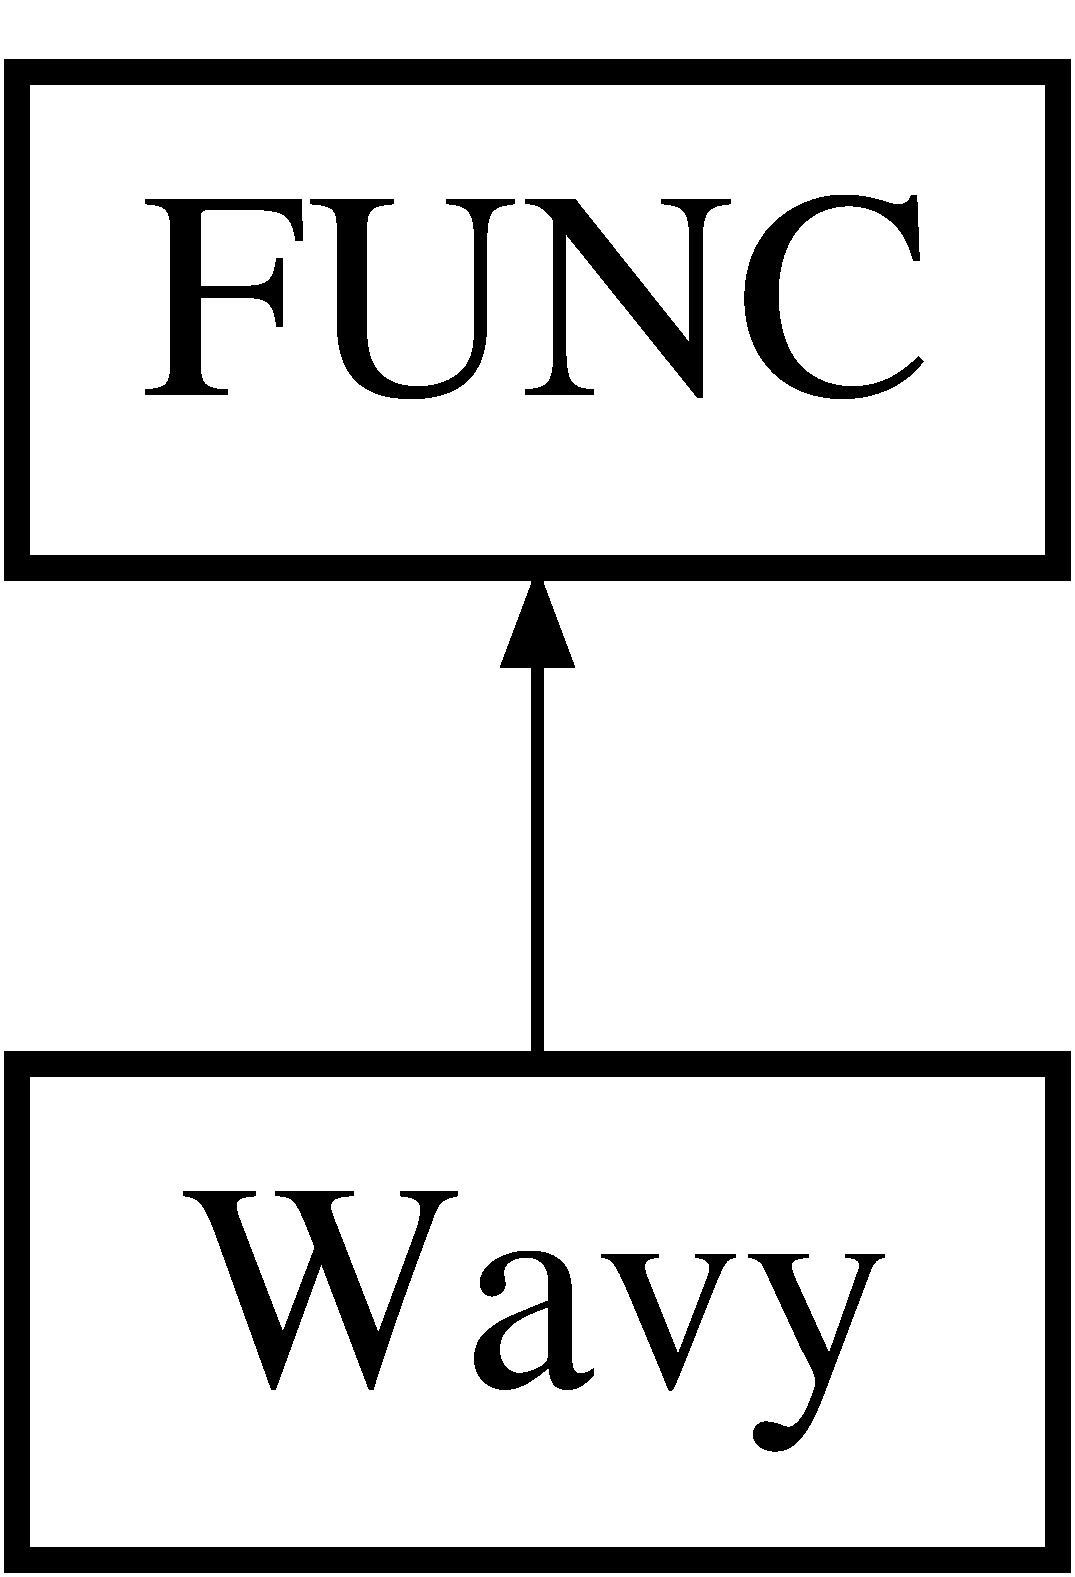
\includegraphics[height=2.000000cm]{class_wavy}
\end{center}
\end{figure}
\subsection*{Public Member Functions}
\begin{DoxyCompactItemize}
\item 
\mbox{\Hypertarget{class_wavy_aec7d22802ab0b2e833f92712266b274c}\label{class_wavy_aec7d22802ab0b2e833f92712266b274c}} 
const double {\bfseries val} (const std\+::vector$<$ double $>$ x)
\item 
\mbox{\Hypertarget{class_wavy_a89817549d743f397812e0c5407f2f3a3}\label{class_wavy_a89817549d743f397812e0c5407f2f3a3}} 
const int \hyperlink{class_wavy_a89817549d743f397812e0c5407f2f3a3}{get\+\_\+dim} (void)
\begin{DoxyCompactList}\small\item\em Virtual method to get value. \end{DoxyCompactList}\end{DoxyCompactItemize}


\subsection{Detailed Description}
Heir of \hyperlink{class_f_u_n_c}{F\+U\+NC} class\+: Wawy function 

The documentation for this class was generated from the following files\+:\begin{DoxyCompactItemize}
\item 
spbsu\+\_\+optimization/F\+U\+N\+C.\+h\item 
spbsu\+\_\+optimization/F\+U\+N\+C.\+cpp\end{DoxyCompactItemize}

%--- End generated contents ---

% Index
\backmatter
\newpage
\phantomsection
\clearemptydoublepage
\addcontentsline{toc}{chapter}{Index}
\printindex

\end{document}
